\newpage
\pageheading{3. Does the same idea help when an object must move?}
The new comparison adds PushT, where a pusher moves a block, and Cube, where
an arm must move the cube to its target. Cube uses the original object-moving
objective. The earlier Cube study measured the gripper reaching a position,
so the two results answer different questions.

Every method uses the same frozen model, cases and required clearance within
a task. We compare planning without a safety check, original SafeCEM, tuned
fixed settings and a feedback controller. The feedback controller can change
how it plans, but cannot shrink the safety buffer. Each final setting has
36 attempts: twelve cases with three planning seeds.

\textbf{PushT, 12-pixel clearance.} Original SafeCEM finishes safely
in 2 of 36 attempts; tuned fixed settings in 19 of 36;
feedback in 20 of 36. Their breach counts are 0,
0 and 0. Tuned fixed settings leave 17 attempts unfinished.

\textbf{Cube, 1 cm clearance.} Original SafeCEM finishes safely
in 0 of 36 attempts; tuned fixed settings in 12 of 36;
feedback in 12 of 36. Their breach counts are 0,
0 and 0. Tuned fixed settings leave 24 attempts unfinished.

\textbf{The lesson.} Better fixed settings help at the same safety requirement.
Feedback's extra benefit remains uncertain. This extension does not test evolution.


\begin{center}
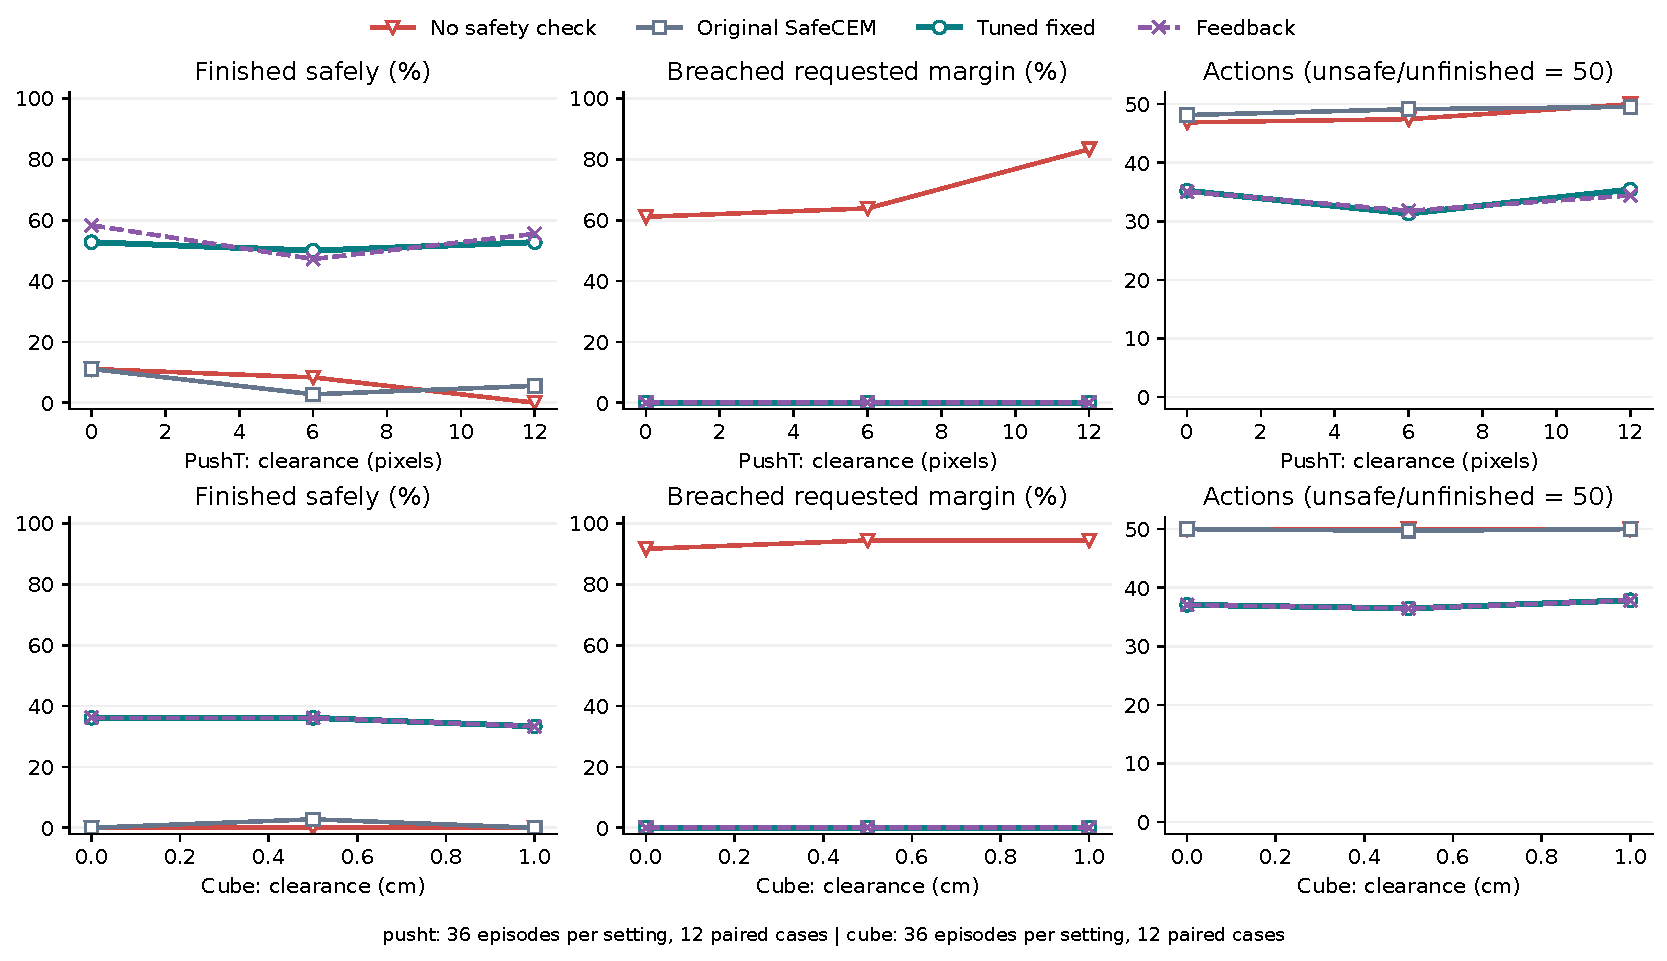
\includegraphics[width=0.90\linewidth]{docs/research/honours-gecco/assets/lewm18-comparison.pdf}
\end{center}

\textbf{What ``faster'' means here.} We count the actions needed to finish
safely. An unsafe or unfinished attempt receives the full 50-action cost.
That stops an early failure from appearing fast. A lower average therefore
means better progress across all attempts. The paper reports actual planning
time separately. The videos are played at a fixed rate and cannot establish
a computation-speed claim.

\textbf{What the safety result covers.} We check the pusher centre or gripper
pinch point against a forbidden area and its extra buffer. We do not certify
the whole arm or the moved object against collision. The Cube cases come from
LeWM's demonstration pairs, rather than the full official OGBench evaluation.

\textbf{The audit matters.} PushT reset moves the simulator slightly. We found
that the first run's checker started from the state before that movement,
corrected the anchor, and repeated the same cases and settings. The first
676 attempts remain preserved and included in the cost, but are excluded
from the final performance estimates above.

\evidence{\href{receipts/18-lewm-results.md}{Task 18 results and accounting};
\href{https://huggingface.co/datasets/Sachioster/SafetyDial-PushT/tree/main/campaigns/lewm18}{PushT data and media};
\href{https://huggingface.co/datasets/Sachioster/SafetyDial-Cube/tree/main/campaigns/lewm18}{Cube data and media}.}
